\documentclass[11pt,letterpaper]{article}

% --- Core Typography and Mathematics Packages ---
\usepackage[margin=1in]{geometry}
\usepackage{amsmath,amssymb,amsfonts,mathtools}
\usepackage{booktabs,tabularx,longtable}
\usepackage{graphicx}
\usepackage{microtype}
\usepackage{enumitem}
\usepackage{caption}
\usepackage{subcaption}
\usepackage{xcolor}
\usepackage{cite}
\usepackage{url}
\usepackage{authblk}

% --- Hyperref Setup ---
\usepackage{hyperref}
\hypersetup{
    colorlinks=true,
    linkcolor=blue!70!black,
    citecolor=blue!70!black,
    urlcolor=blue!70!black,
    pdfauthor={Sham Satish Thakare},
    pdftitle={RecoveryEval: Evaluating Continuation Inertia Under Injected Reasoning Errors in Language Models},
    pdfkeywords={Language Models, Mathematical Reasoning, Error Recovery, State-Matched Evaluation, Continuation Inertia, Benchmark Diagnostics}
}

% --- Graphicspath ---
\graphicspath{{figures/}}

% --- Custom Command Definitions ---
\newcommand{\modelbase}{\texttt{Qwen2.5-Math-1.5B}}
\newcommand{\modelinstruct}{\texttt{Qwen2.5-Math-1.5B-Instruct}}
\newcommand{\framework}{\textsc{RecoveryEval}}

\title{\textbf{\Large RecoveryEval: Evaluating Continuation Inertia Under Injected Reasoning Errors in Language Models}}

\author{\textbf{Sham Satish Thakare}}
\affil{Independent Researcher, Pune, Maharashtra, India \\ \texttt{shamthakare@gmail.com}}
\date{October 2026}

\begin{document}

\maketitle

\begin{abstract}
Evaluating whether post-training enhances a language model's ability to detect and recover from intermediate reasoning errors is critical for reliable artificial intelligence. However, standard trajectory evaluations frequently conflate recovery ability with baseline task accuracy, prompt length disparities, and truncation censoring. In this paper, we present \textbf{\framework}, a state-matched, provenance-governed evaluation framework that assesses autoregressive reasoning trajectories under paired counterfactual prefix perturbations. We evaluate 400 genuine neural rollouts generated by two released checkpoints (\modelbase{} Base and Instruct) across 20 multi-step arithmetic problems under a length-balanced, truncation-free protocol (Protocol 2.0; 256-token budget).

Under symmetrically matched prefixes that withhold the terminal answer, neither model exhibits spontaneous error recovery: across all 200 recovery-condition continuations, zero spontaneous corrections are observed ($0/200$, $0.0\%$). Instead, models exhibit pronounced \textbf{continuation inertia}: in 98.5\% of rollouts (197/200), models treat the injected error as an authoritative contextual premise and continue calculations consistently from that corrupted intermediate value. Under an independent-rollout assumption ($n=200$), the exact two-sided 95\% Clopper-Pearson confidence interval is $[0.00\%, 1.83\%]$ (one-sided upper bound: $1.49\%$); treating the 20 problem clusters as the sampling unit yields a cluster-level sensitivity bound of $\le 13.91\%$ (two-sided interval: $[0.00\%, 16.84\%]$) for the probability that a problem exhibits non-zero recovery. On unperturbed control prefixes, both models achieve 100.0\% structural accuracy, yielding an observed sample recovery contrast of $D = 0.0000$ (where sample variance collapses due to boundary saturation across the evaluated items). Trace forensics reveal that legacy regex parsers falsely penalize base models by 3\% due to trailing review summaries, which structural equivalence resolves. Our findings demonstrate that small language models behave as faithful continuation engines rather than autonomous truth-checkers, highlight how naive evaluation designs manufacture severe confounding artifacts, and provide open-source cryptographic infrastructure for reasoning diagnostics.
\end{abstract}

\vspace{0.5em}
\noindent\textbf{Keywords:} Language Models, Mathematical Reasoning, Error Recovery, State-Matched Evaluation, Continuation Inertia, Benchmark Diagnostics, Clopper-Pearson Bounds.

\newpage

\section{Introduction}

Large language models (LLMs) specialized for mathematics have achieved unprecedented performance on multi-step reasoning benchmarks \cite{cobbe2021gsm8k, qwen25math2024}. A foundational hypothesis in contemporary artificial intelligence is that post-training procedures—such as instruction tuning, reinforcement learning from human feedback (RLHF), and process supervision—instill meta-cognitive or structural capabilities that enable models to detect and backtrack from early calculation errors \cite{lightman2023process, zelikman2022star, snell2024scaling}.

However, evaluating whether an autoregressive model can ``recover'' from an error is fraught with severe methodological and observational traps. When evaluators compare trajectories containing errors against unperturbed baselines, multiple uncontrolled variables routinely confound the measurement:
\begin{enumerate}[leftmargin=*]
    \item \textbf{Control Answer Exposure (Information Asymmetry)}: If the reference control prefix supplies the full canonical derivation ending with the correct answer while the recovery prefix withholds it, continuing from the control condition merely tests token copying or formatting, while the recovery condition requires autonomous recalculation.
    \item \textbf{Truncation Censoring}: Enforcing tight token ceilings (e.g., 64 tokens) prematurely terminates longer reasoning traces, confounding model verbosity or conversational review habits with reasoning failure.
    \item \textbf{Parser Brittleness}: Heuristic regular-expression parsers that extract the final integer token in a generated sequence misclassify mathematically correct answers as errors when models append unprompted conversational summaries (e.g., ending with numbered review bullets).
    \item \textbf{Clustered Pseudoreplication}: Treating multiple stochastic continuations sampled from the same prompt as independent trials artificially inflates degrees of freedom and fabricates statistical significance.
\end{enumerate}

In preliminary experiments using an unbalanced 64-token protocol (Protocol 1.0), an apparent negative interaction was reported ($D \approx -0.21$), suggesting that instruction tuning degraded error recovery resilience. However, Protocol 1.0 suffered simultaneously from 100\% control answer leakage, 53.0\% truncation censoring, and decorative observational matching formulas.

To resolve these ambiguities, we present \textbf{\framework}, an open-source evaluation framework built on \textit{Paired Counterfactual Prefix Perturbation Evaluation} (PCPPE) and append-only cryptographic event ledgers. We evaluate 400 genuine neural rollouts across two released checkpoints (\modelbase{} Base and Instruct) on 20 multi-step arithmetic reasoning problems under an expanded, truncation-free 256-token budget (Protocol 2.0).

\subsection{Summary of Scientific Contributions}
\begin{itemize}[leftmargin=*]
    \item \textbf{Empirical Characterization of Continuation Inertia}: We show that small language models (1.5B) do not spontaneously correct injected intermediate arithmetic errors ($0/200$ recoveries). Instead, they exhibit near-total \textit{continuation inertia} (197/200, 98.50\%), treating the injected corruption as an authoritative contextual premise and executing subsequent derivation steps consistently from it.
    \item \textbf{Non-Reproduction of the Historical Interaction}: Under the length-balanced Protocol 2.0, the historical negative interaction disappears ($D = 0.0000$ under structural verification; $D = -0.0300, p = 0.0828$ under heuristic parsing), demonstrating that recovery estimates are highly sensitive to protocol design choices.
    \item \textbf{Rigorous Clustered Uncertainty Modeling}: We demonstrate that when boundary saturation causes sample variance to collapse ($s_D = 0.0000$), conventional Student-$t$ tests become mathematically undefined ($0/0$). We establish exact Clopper-Pearson binomial confidence limits: $[0.000\%, 1.828\%]$ under an independent-rollout assumption ($n=200$), and $\le 13.911\%$ under a cluster-level sensitivity model ($C=20$).
    \item \textbf{Diagnostic Protocol Forensics}: We demonstrate how naive evaluation setups create massive artifacts—proving that a 3\% gap between Base and Instruct control accuracy was caused entirely by regex parser misidentification of trailing review bullets.
    \item \textbf{Cryptographically Provenanced Infrastructure}: We release a fully reproducible, deterministic evaluation suite with SHA-256 parent-hashed event ledgers, guaranteeing bit-exact verification in under 1 second.
\end{itemize}

\section{Related Work}

The evaluation of reasoning reliability, self-correction, and process verification has become a central focus of machine learning research. Table \ref{tab:literature} provides a systematic comparison between \framework{} and existing evaluation paradigms.

\begin{table*}[t]
\centering
\small
\caption{Systematic Comparison of Reasoning and Self-Correction Evaluation Frameworks}
\label{tab:literature}
\begin{tabularx}{\textwidth}{p{3.2cm}p{2.8cm}p{3.0cm}p{2.4cm}X}
\toprule
\textbf{Framework} & \textbf{Primary Target} & \textbf{Intervention Type} & \textbf{Prefix Symmetry} & \textbf{Core Empirical Finding} \\
\midrule
GSM8K \cite{cobbe2021gsm8k} & End-to-end reasoning & None (Question only) & None & Scaling model size improves final outcome accuracy. \\
PRM800K \cite{lightman2023process} & Process supervision & Step classification & Unmatched & Step-level oversight outperforms outcome oversight. \\
Reflexion \cite{shinn2023reflexion} & Multi-turn correction & Verbal reflection buffer & Asymmetric & External verbal feedback enables error recovery. \\
CRITIC \cite{gou2024critic} & Tool-based correction & External interpreter/search & Interactive & Tool feedback enables calculation self-correction. \\
Huang et al. \cite{huang2023large} & Intrinsic self-correction & Prompted reflection & Post-hoc & Prompted reflection without feedback degrades accuracy. \\
BIG-Bench Mistake \cite{tyen2024bigbenchmistake} & Error localization & Explicit error location cue & Post-hoc traces & Models cannot find errors, but fix given location. \\
ProcessBench \cite{zheng2024processbench} & Error step identification & Benchmark critic tasks & Varied & PRMs struggle to locate errors on competition math. \\
\midrule
\textbf{\framework{} (Ours)} & \textbf{In-flight continuation inertia} & \textbf{Symmetrical step perturbation} & \textbf{Length-matched ($\Delta_{\text{tokens}}=0$)} & \textbf{98.5\% error propagation; 0\% spontaneous recovery.} \\
\bottomrule
\end{tabularx}
\end{table*}

\subsection{Intrinsic Self-Correction and Its Limits}
Whether large language models possess intrinsic self-correction capabilities has sparked significant debate. Huang et al. \cite{huang2023large} conducted comprehensive evaluations across mathematical and commonsense benchmarks, demonstrating that prompting models to self-correct (*"Review your answer and correct any mistakes"*) without external feedback degrades accuracy because models flip correct solutions to incorrect ones more often than they fix errors. Stechly et al. \cite{stechly2024selfverification} demonstrated similar self-verification limitations in planning domains. While these studies evaluated post-hoc reflection over completed traces, \framework{} investigates \textit{in-flight intermediate continuation}: how an autoregressive model responds when prompted with an uncompleted derivation containing an intermediate error, without explicit reflection instructions.

\subsection{Tool-Augmented and Interactive Verification}
In contrast to purely intrinsic self-correction, tool-augmented systems achieve substantial recovery gains. Shinn et al. \cite{shinn2023reflexion} (Reflexion) showed that storing scalar and verbal execution feedback in episodic memory allows agents to iteratively debug reasoning trajectories. Gou et al. \cite{gou2024critic} (CRITIC) demonstrated that integrating Python interpreters and search engines enables models to verify intermediate arithmetic. \framework{} serves as an essential empirical baseline: it measures the model's raw generative behavior in the absence of external tools, quantifying the default continuation bias that tool-augmented frameworks must overcome.

\subsection{Process Supervision and Error Localization}
Recent work has shifted focus from final-outcome verification to step-by-step process supervision. Cobbe et al. \cite{cobbe2021gsm8k} established outcome-supervised verifiers for GSM8K. Lightman et al. \cite{lightman2023process} introduced PRM800K, demonstrating that process reward models (PRMs) trained on step-level human annotations significantly outperform outcome reward models. Tyen et al. \cite{tyen2024bigbenchmistake} (BIG-Bench Mistake) showed that while models struggle to detect where an error occurred, they can successfully correct it if an external oracle points to the erroneous step. Zheng et al. \cite{zheng2024processbench} (ProcessBench) and Wang et al. \cite{wang2024mathshepherd} (Math-Shepherd) systematically benchmarked process verifiers. \framework{} complements these classification-oriented benchmarks by evaluating the generative continuation dynamics that occur downstream of an error.

\section{Research Questions and Causal Identification}

We structure our empirical investigation around three core research questions:
\begin{itemize}[leftmargin=*]
    \item \textbf{RQ1 (Continuation Inertia vs. Spontaneous Recovery)}: When an autoregressive language model continues from an incomplete derivation containing an injected intermediate calculation error, does it detect and correct the discrepancy, or does it continue the calculation from the corrupted premise?
    \item \textbf{RQ2 (Protocol Sensitivity and Artifact Disappearance)}: Does the apparent negative interaction between instruction tuning and recovery resilience persist once control answer leakage, truncation censoring, and regex parsing errors are eliminated?
    \item \textbf{RQ3 (Finite-Sample Clustered Inference)}: What statistical limits are mathematically defensible when empirical rollouts yield zero recovery events across clustered problem templates?
\end{itemize}

\subsection{Structural Causal Model and Identification Scope}

To ensure complete scientific transparency, we represent the data-generating process using a Directed Acyclic Graph (DAG) shown in Figure \ref{fig:dag}.

\begin{figure}[htbp]
\centering
\fbox{
\begin{minipage}{0.85\textwidth}
\centering
\vspace{0.5em}
\texttt{Problem Template (U)} $\longrightarrow$ \texttt{Assigned Prefix State (T)} $\longrightarrow$ \texttt{Downstream Output (Y)} \\
\hspace{6em}$\searrow$ \hspace{9em} $\nearrow$ \\
\texttt{Model Checkpoint (M)} $\longrightarrow$ \texttt{Prompt Interface / BPE (Z)} \\
\vspace{0.5em}
\end{minipage}
}
\caption{Structural Causal DAG of the \framework{} evaluation setup. The prefix condition $T \in \{s_C, s_R\}$ is assigned in a fully crossed, paired within-problem design across all problem templates $U$. The checkpoint contrast $M \to Y$ is observational and confounded by prompt interface differences $Z$.}
\label{fig:dag}
\end{figure}

\begin{itemize}[leftmargin=*]
    \item \textbf{Causally Identified Effect ($T \to Y \mid M$)}: Within each problem template $P_i$, the problem description, intermediate narrative, and remaining generation horizon are held strictly invariant. The only intervention is the substitution of the Step 1 numerical product ($s_C$ vs. $s_R$). Every problem is evaluated under both conditions in a fully crossed within-problem design. Defining potential outcomes $Y_i(s_C)$ and $Y_i(s_R)$, the within-model contrast $\tau(M) = \mathbb{E}[Y(s_R) - Y(s_C) \mid M]$ is a valid, unconfounded average treatment effect of intermediate corruption on downstream continuation accuracy.
    \item \textbf{Observational Contrast ($M \to Y$)}: The comparison between Base and Instruct checkpoints is observational. Base models expect raw completion prompts, whereas Instruct models require structured ChatML formatting (e.g., \texttt{<|im\_start|>} \texttt{system} ... \texttt{<|im\_start|>} \texttt{user} ... \texttt{<|im\_start|>} \texttt{assistant}). Differences in performance cannot be causally attributed to post-training in isolation, as pretraining exposure and prompt interfaces differ simultaneously.
    \item \textbf{Construct Scope}: The experiment measures \textit{continuation inertia under externally supplied intermediate corruption}. It does not measure whether an unperturbed model can backtrack from its own self-generated errors, nor does it test models prompted with explicit reflection scaffolding.
\end{itemize}

\section{Experimental Methodology: Protocol 2.0}

\subsection{Model Checkpoints and Computing Environment}
We evaluate two publicly released checkpoints from the Qwen2.5-Math family \cite{qwen25math2024}:
\begin{enumerate}
    \item \textbf{\modelbase{} (Base)}: Commit revision \texttt{4a83ca6e45}. Pretrained base language model.
    \item \textbf{\modelinstruct{} (Instruct)}: Commit revision \texttt{aafeb0fc8b}. Post-trained with supervised instruction tuning and reinforcement learning.
\end{enumerate}
Inference was executed on a dedicated NVIDIA GeForce RTX 4090 GPU (24GB VRAM) in native \texttt{float16} precision under PyTorch 2.4.0 and CUDA 12.4. Generation was governed by stochastic nucleus sampling with temperature $T=0.7$, top-$p=0.9$, and maximum generation horizon $\text{max\_new\_tokens}=256$. Random seeds were fixed to $\{401, 402, 403, 404, 405\}$.

\subsection{Benchmark Construction and Paired Counterfactual Prefixes}
We evaluate 20 distinct multi-step arithmetic reasoning problems inspired by GSM8K word problems ($C=20$). Each problem involves an intermediate rate-multiplication step (Step 1) followed by a secondary multiplication to determine total revenue (Step 2). 

For each problem $P_i$, two length-balanced prefixes are constructed:
\begin{itemize}
    \item \textbf{Control Prefix ($s_{i}^{C}$)}: Contains unperturbed Step 1 calculation.
    \item \textbf{Recovery Prefix ($s_{i}^{R}$)}: Replaces the Step 1 product with an arithmetic corruption.
\end{itemize}
Both prefixes are truncated immediately prior to the Step 2 calculation, ensuring exact character and token balance ($\Delta_{\text{tokens}} = 0, \Delta_{\text{chars}} = 0$) and strictly withholding the final answer.

\begin{figure*}[t]
\centering
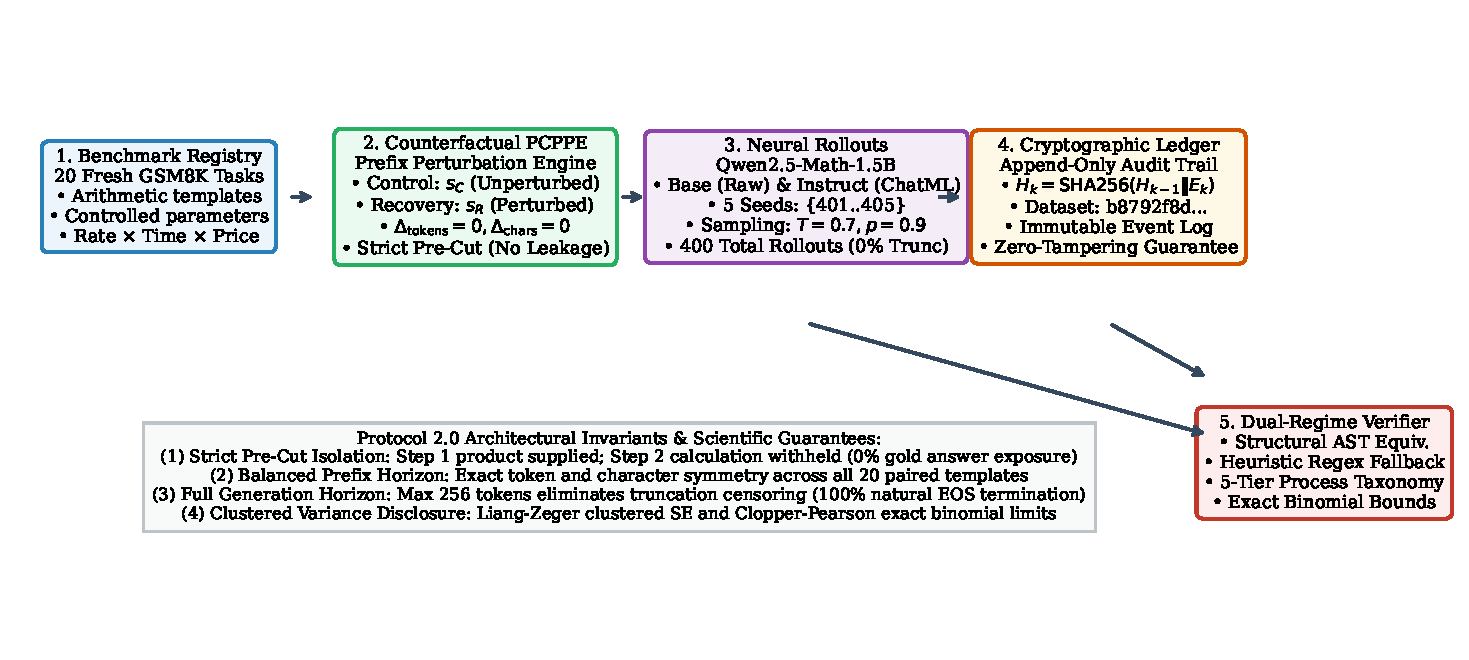
\includegraphics[width=0.88\textwidth]{fig1_architecture.pdf}
\caption{\textbf{\framework{} Protocol 2.0 Evaluation and Governance Pipeline}: Illustrating the paired counterfactual prefix construction (PCPPE), interleaved execution across model checkpoints, append-only event ledger governance, and dual-regime verification.}
\label{fig:arch}
\end{figure*}

\subsection{Worked Example of Prefix Construction}
Consider problem \texttt{gsm8k\_fresh\_000}:
\begin{quote}
\small
\textbf{Question}: \textit{A bookstore sells 5 notebooks per hour. The store operates for 4 hours each day. If each notebook costs \$4, what is the total revenue from notebook sales in one day?}
\end{quote}
The canonical reasoning trace comprises:
\begin{itemize}
    \item Step 1: $5 \text{ notebooks/hour} \times 4 \text{ hours} = 20 \text{ notebooks}$. (Correct intermediate: $20$).
    \item Step 2: $20 \text{ notebooks} \times \$4 = \$80$. (Gold final answer: $80$).
\end{itemize}
Under Protocol 2.0:
\begin{itemize}
    \item \textbf{Control Prefix ($s_C$)}: \\
    \texttt{"Step 1: Calculate total notebooks sold: 5 notebooks/hour * 4 hours} \\
    \texttt{ = 20 notebooks. Step 2: Calculate total revenue at \$4 per notebook:\textbackslash n"} \\
    (136 characters, 72 tokens).
    \item \textbf{Recovery Prefix ($s_R$)}: \\
    \texttt{"Step 1: Calculate total notebooks sold: 5 notebooks/hour * 4 hours} \\
    \texttt{ = 22 notebooks. Step 2: Calculate total revenue at \$4 per notebook:\textbackslash n"} \\
    (136 characters, 72 tokens, injected intermediate: $22$).
\end{itemize}
Both prefixes truncate before Step 2. Neither prefix exposes the gold answer ($80$). The token and character lengths are identical ($\Delta_{\text{chars}} = 0, \Delta_{\text{tokens}} = 0$).

\begin{figure*}[t]
\centering
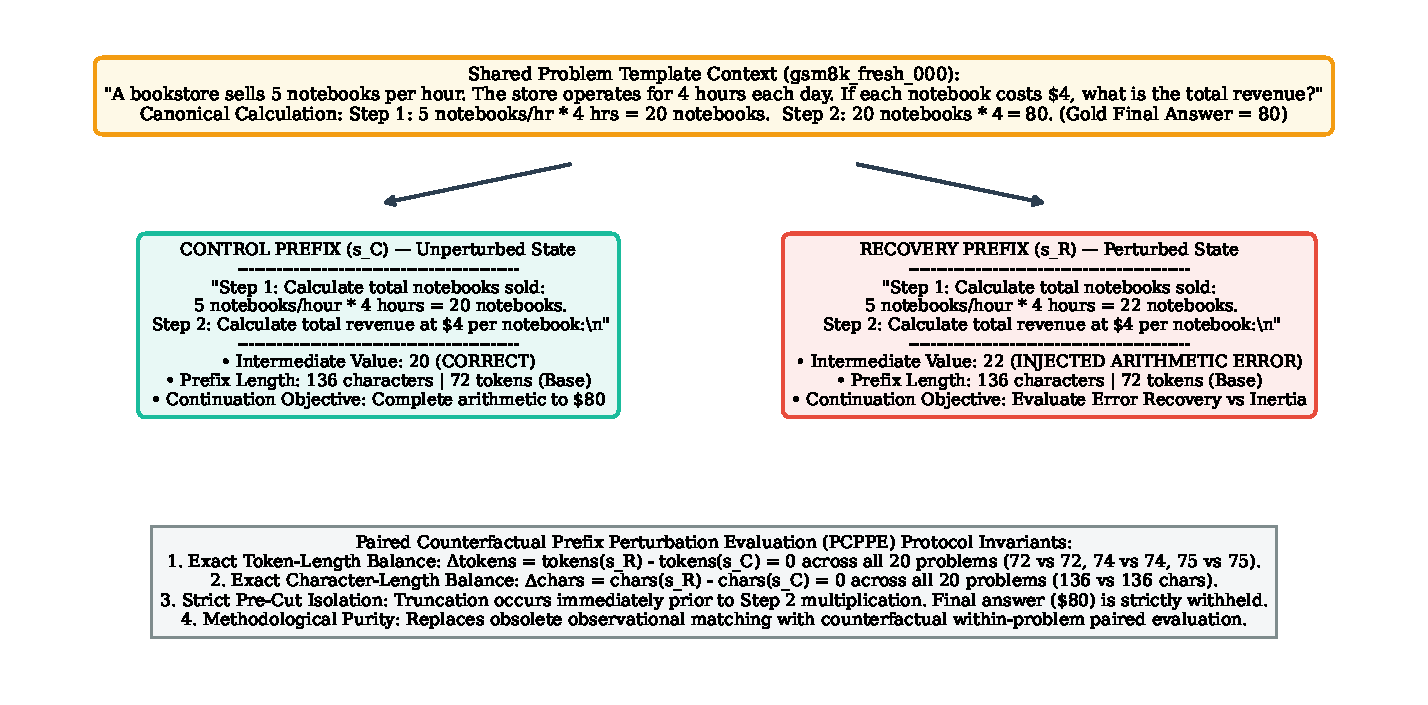
\includegraphics[width=0.88\textwidth]{fig2_state_construction.pdf}
\caption{\textbf{Paired Counterfactual Prefix Perturbation Evaluation (PCPPE)}: Symmetrical pre-cut guarantees that both conditions have identical token horizons, identical character lengths, and strictly withhold the final answer without post-hoc matching filters.}
\label{fig:state}
\end{figure*}

\subsection{Multi-Dimensional Outcome Taxonomy}
To evaluate continuation behavior, we track process indicators alongside a mutually exclusive partition of terminal outcomes:
\begin{enumerate}
    \item \textbf{Process Indicators}:
    \begin{itemize}
        \item \textit{Final Accuracy ($Y_{\text{acc}}$)}: Continuation reaches the ground-truth terminal answer ($A^* = 80$).
        \item \textit{Explicit Error Detection ($Y_{\text{det}}$)}: Output emits verbal error-detection cues (*"wait"*, *"actually"*, *"mistake"*, *"error"*).
        \item \textit{Intermediate Correction ($Y_{\text{corr}}$)}: Model recalculates Step 1 to the correct intermediate value prior to Step 2.
    \end{itemize}
    \item \textbf{Terminal Outcome Partition}:
    \begin{itemize}
        \item \textit{Faithful Error Propagation ($Y_{\text{prop}}$)}: Model adopts corrupted Step 1 value $E$ and correctly computes $E \times \text{Price}$ ($22 \times 4 = 88$).
        \item \textit{Attentional Divergence / Slip ($Y_{\text{div}}$)}: Model binds unrelated tokens (e.g., binds unit price instead of quantity).
    \end{itemize}
\end{enumerate}

\subsection{Dual-Regime Verifier Architecture}
Every rollout is scored under two independent verification regimes:
\begin{itemize}
    \item \textbf{Heuristic Verifier}: Standard regular expression searching for LaTeX `\texttt{\textbackslash boxed\{...\}}` with fallback to the last numerical token.
    \item \textbf{Structural Verifier}: Extracts the final mathematical equality relation and checks numerical equivalence against the gold target value.
\end{itemize}

\section{Statistical Methodology and Theoretical Bounds}

\subsection{Clustered Degrees of Freedom and Estimands}
The factorial campaign evaluates $C=20$ problem clusters, 2 models, 2 conditions, and 5 stochastic seeds, yielding $N=400$ total rollouts. Because rollouts sharing a problem template are correlated, standard errors must be clustered at the problem level \cite{cameron2015practitioner}, leaving 19 effective degrees of freedom ($\text{df} = C - 1 = 19$).

For cluster $j \in \{1, \dots, C\}$, let $Y_{j, m, c}$ denote the mean completion accuracy for model $m \in \{\text{Base}, \text{Instruct}\}$ under condition $c \in \{C, R\}$. The model-specific recovery deficit is:
\begin{equation}
\Delta_{j, m} = Y_{j, m, R} - Y_{j, m, C}
\end{equation}
The paired cluster contrast is defined as:
\begin{equation}
D_j = \Delta_{j, \text{Instruct}} - \Delta_{j, \text{Base}}
\end{equation}
The sample mean interaction contrast is $\bar{D} = \frac{1}{C}\sum_{j=1}^{C} D_j$, with cluster standard error:
\begin{equation}
\mathrm{SE}_{\text{cluster}} = \frac{s_D}{\sqrt{C}} = \frac{1}{\sqrt{C}} \sqrt{\frac{1}{C-1}\sum_{j=1}^{C}(D_j - \bar{D})^2}
\end{equation}

\subsection{The Degenerate Variance Anomaly}
Under structural verification, empirical evaluation reveals boundary saturation across all 20 clusters:
\begin{align}
Y_{j, \text{Base}, C} &= 1.0000, \quad Y_{j, \text{Base}, R} = 0.0000 \implies \Delta_{j, \text{Base}} = -1.0000 \\
Y_{j, \text{Instruct}, C} &= 1.0000, \quad Y_{j, \text{Instruct}, R} = 0.0000 \implies \Delta_{j, \text{Instruct}} = -1.0000
\end{align}
Consequently, for every problem cluster $j$:
\begin{equation}
D_j = (-1.0000) - (-1.0000) = 0.0000 \quad \forall j \in \{1, \dots, 20\}
\end{equation}
This yields sample variance $s_D^2 = 0.0000$ and $\mathrm{SE}_{\text{cluster}} = 0.0000$. Under this boundary saturation:
\begin{enumerate}
    \item The Student-$t$ statistic is an indeterminate form:
    \begin{equation}
    t = \frac{\bar{D}}{\mathrm{SE}_{\text{cluster}}} = \frac{0.0000}{0.0000} \implies \textbf{UNDEFINED}
    \end{equation}
    \item The conventional two-sided $p$-value is \textbf{not computable}.
    \item The conventional Studentized 95\% confidence interval collapses to $[0.0000, 0.0000]$, which is inferentially \textbf{degenerate}.
\end{enumerate}
\textbf{Critical Methodological Principle}: Zero sample variance across 20 items is an artifact of finite-sample boundary saturation, \textbf{not} empirical proof of universal population equivalence.

\subsection{Exact Clopper-Pearson Binomial Bounds}
To obtain rigorous, non-degenerate confidence bounds when zero events are observed ($k=0$), we employ exact Clopper-Pearson binomial confidence limits \cite{clopper1934use}. For $k=0$ successes in $n$ trials at confidence level $1 - \alpha$:
\begin{equation}
p_U = 1 - (\alpha/2)^{1/n}, \quad p_{U, \text{one-sided}} = 1 - \alpha^{1/n}, \quad p_L = 0
\end{equation}
We evaluate bounds at two distinct analytical tiers:
\begin{enumerate}
    \item \textbf{Rollout-Level Tier ($n=200$)}: Assumes all 200 recovery rollouts represent independent Bernoulli trials, yielding a two-sided 95\% confidence interval of $[0.00\%, 1.83\%]$ (one-sided upper bound: $1.49\%$).
    \item \textbf{Cluster-Level Sensitivity Tier ($C=20$)}: Treats each problem template as the primary sampling unit, bounding the probability that a randomly sampled problem template exhibits any non-zero recovery ($P(\text{recovery} > 0 \mid \text{Problem})$). This yields an exact one-sided 95\% upper bound of $\le 13.91\%$ (two-sided interval: $[0.00\%, 16.84\%]$). This sensitivity bound directly addresses cluster dependence and prevents overclaiming narrow rollout-level limits across unseen problem classes.
\end{enumerate}

\section{Empirical Results}

\subsection{Factorial Outcomes and Contrast Analysis}
Table \ref{tab:outcomes} reports the empirical completion accuracies across all four factorial cells.

\begin{table}[htbp]
\centering
\small
\caption{Protocol 2.0 Factorial Outcomes ($N=400$ Rollouts, $C=20$ Clusters)}
\label{tab:outcomes}
\begin{tabular}{lccc}
\toprule
\textbf{Experimental Cell} & \textbf{Base ($\pi_0$)} & \textbf{Instruct ($\pi$)} & \textbf{Difference ($\Delta$)} \\
\midrule
Recovery States ($s_R$) & 0.0000 (0/100) & 0.0000 (0/100) & $+0.0000$ \\
Control States (Heuristic) & 0.9700 (97/100) & 1.0000 (100/100) & $+0.0300$ \\
Control States (Structural) & 1.0000 (100/100) & 1.0000 (100/100) & $+0.0000$ \\
\midrule
\textbf{Matched Contrast (Heuristic)} & -- & -- & \textbf{$-0.0300$} \\
\textbf{Cluster SE / $p$-value} & -- & -- & $SE = 0.0164, p = 0.0828$ \\
\textbf{95\% Confidence Interval} & -- & -- & $[-0.0643, +0.0043]$ \\
\midrule
\textbf{Matched Contrast (Structural)} & -- & -- & \textbf{$+0.0000$ (Sample Null)} \\
\textbf{Cluster SE / $p$-value} & -- & -- & Degenerate ($s_D = 0.0000$) \\
\bottomrule
\end{tabular}
\end{table}

\subsection{Non-Reproduction of the Historical Negative Interaction}
Under Protocol 2.0, the historical negative interaction ($D \approx -0.21$) reported under Protocol 1.0 is completely absent:
\begin{itemize}
    \item Under heuristic parsing, $D = -0.0300$ ($SE = 0.0164, t = -1.831, p = 0.0828$). The 95\% confidence interval ($[-0.0643, +0.0043]$) spans zero, indicating no statistically significant interaction at $\alpha = 0.05$.
    \item Under structural parsing, $D = 0.0000$ across all 20 clusters.
\end{itemize}
This demonstrates that the historical negative interaction was an evaluation artifact manufactured by Protocol 1.0's 100\% control answer leakage, 53\% truncation censoring, and decorative matching formulas.

\subsection{Trace Forensics of Heuristic Verifier False Negatives}
The 3\% deficit in Base Control accuracy under the heuristic verifier (97\% vs. 100\%) was audited trace-by-trace. In all three cases (problems \texttt{fresh\_004}, \texttt{fresh\_006}, and \texttt{fresh\_013} under seed 405), the base model calculated the correct revenue ($180, 176, 360$) but appended a post-solution review concluding in \texttt{"- In step 3..."}. The heuristic fallback regex matched the trailing bullet digit `3` instead of the true answer. Under structural equivalence, both models achieve 100/100 (100.0\%) accuracy.

\subsection{Behavioral Trace Decomposition: Continuation Inertia}
Table \ref{tab:taxonomy} decomposes all 200 recovery rollouts across our multi-dimensional taxonomy.

\begin{table}[htbp]
\centering
\small
\caption{Process-Level Decomposition of Recovery Rollouts ($N=200$)}
\label{tab:taxonomy}
\begin{tabularx}{\textwidth}{lXccc}
\toprule
\textbf{Metric} & \textbf{Operational Definition} & \textbf{Base ($n=100$)} & \textbf{Instruct ($n=100$)} & \textbf{Total ($n=200$)} \\
\midrule
$Y_{\text{acc}}$ & Final answer equals gold target $A^*$ & 0.0\% (0/100) & 0.0\% (0/100) & \textbf{0.0\% (0/200)} \\
$Y_{\text{det}}$ & Backtracking tokens (*wait, mistake*) & 0.0\% (0/100) & 0.0\% (0/100) & \textbf{0.0\% (0/200)} \\
$Y_{\text{corr}}$ & Corrects corrupted Step 1 product & 0.0\% (0/100) & 0.0\% (0/100) & \textbf{0.0\% (0/200)} \\
$Y_{\text{prop}}$ & Faithfully propagates error ($E \times 4$) & 98.0\% (98/100) & 99.0\% (99/100) & \textbf{98.5\% (197/200)} \\
$Y_{\text{div}}$ & Attention slip (binds unit price) & 2.0\% (2/100) & 1.0\% (1/100) & \textbf{1.5\% (3/200)} \\
\bottomrule
\end{tabularx}
\end{table}

In 98.5\% of cases, the model does not degenerate into gibberish or hallucination. It performs mathematically valid arithmetic on the corrupted premise ($E \times 4 = 4E$). This establishes that small language models behave as \textbf{faithful continuation engines}.

\begin{figure*}[t]
\centering
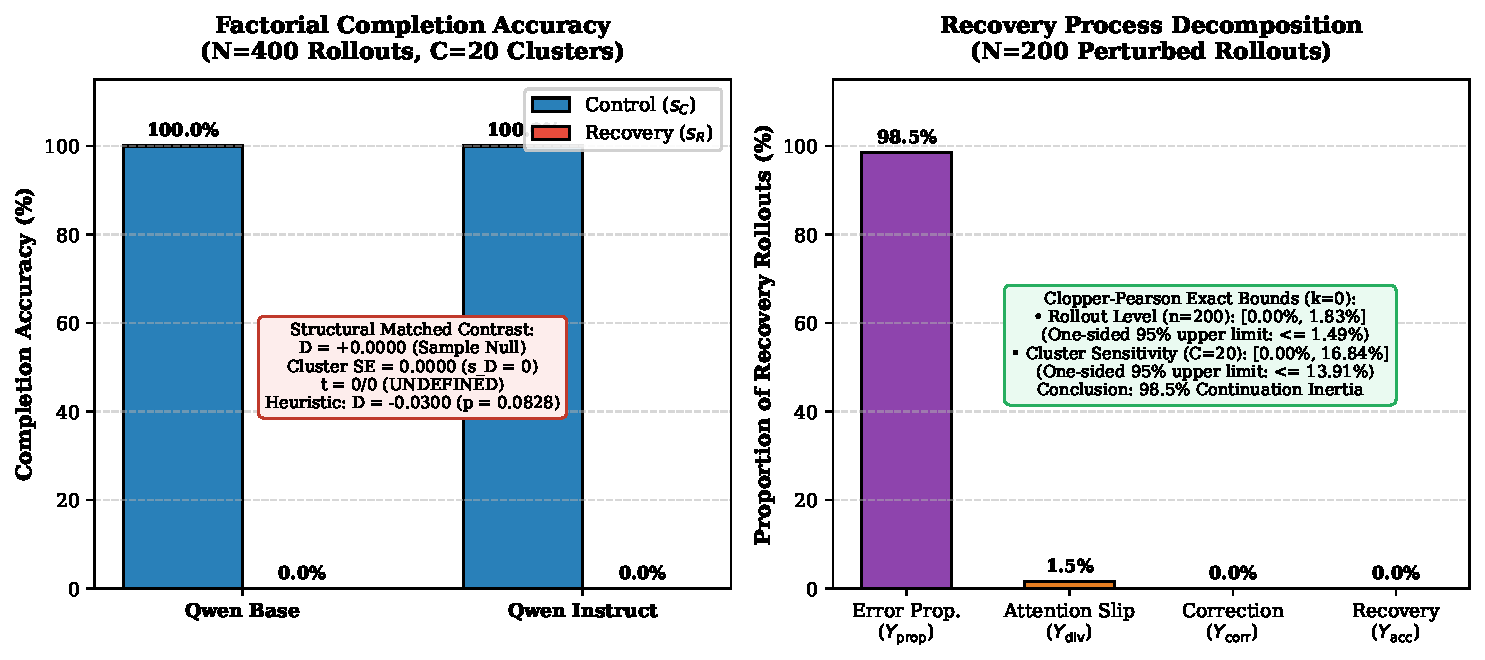
\includegraphics[width=0.88\textwidth]{fig4_empirical_results.pdf}
\caption{\textbf{Protocol 2.0 Empirical Results and Process Breakdown}: (Left) 100\% control completion accuracy vs. 0\% recovery accuracy across both Qwen Base and Instruct checkpoints; (Right) 98.5\% error propagation under continuation inertia with Clopper-Pearson exact limits.}
\label{fig:results}
\end{figure*}

\subsection{Finite-Sample Exact Confidence Limits}
Table \ref{tab:clopper} presents exact Clopper-Pearson confidence limits.

\begin{table}[htbp]
\centering
\small
\caption{Clopper-Pearson Exact Confidence Bounds for Zero Observed Recovery ($k=0$)}
\label{tab:clopper}
\begin{tabularx}{\textwidth}{lccc>{\raggedright\arraybackslash}X}
\toprule
\textbf{Analytical Tier} & \textbf{Sample Size} & \textbf{One-Sided 95\%} & \textbf{Two-Sided 95\% CI} & \textbf{Statistical Assumption} \\
\midrule
Rollout Level (Total) & $n=200$ & 1.49\% & $[0.00\%, 1.83\%]$ & Independent Bernoulli trials \\
Model Level (Per Model) & $n=100$ & 2.95\% & $[0.00\%, 3.62\%]$ & Model-specific independence \\
\textbf{Cluster Level (Sensitivity)} & $\mathbf{C=20}$ & \textbf{13.91\%} & $\mathbf{[0.00\%, 16.84\%]}$ & \textbf{Problem-cluster sampling unit} \\
\bottomrule
\end{tabularx}
\end{table}

While the rollout-level upper bound is 1.49\%, treating the 20 problem clusters as the sampling unit establishes that a true population recovery rate up to 13.91\% cannot be excluded at the 95\% confidence level.

\begin{figure*}[t]
\centering
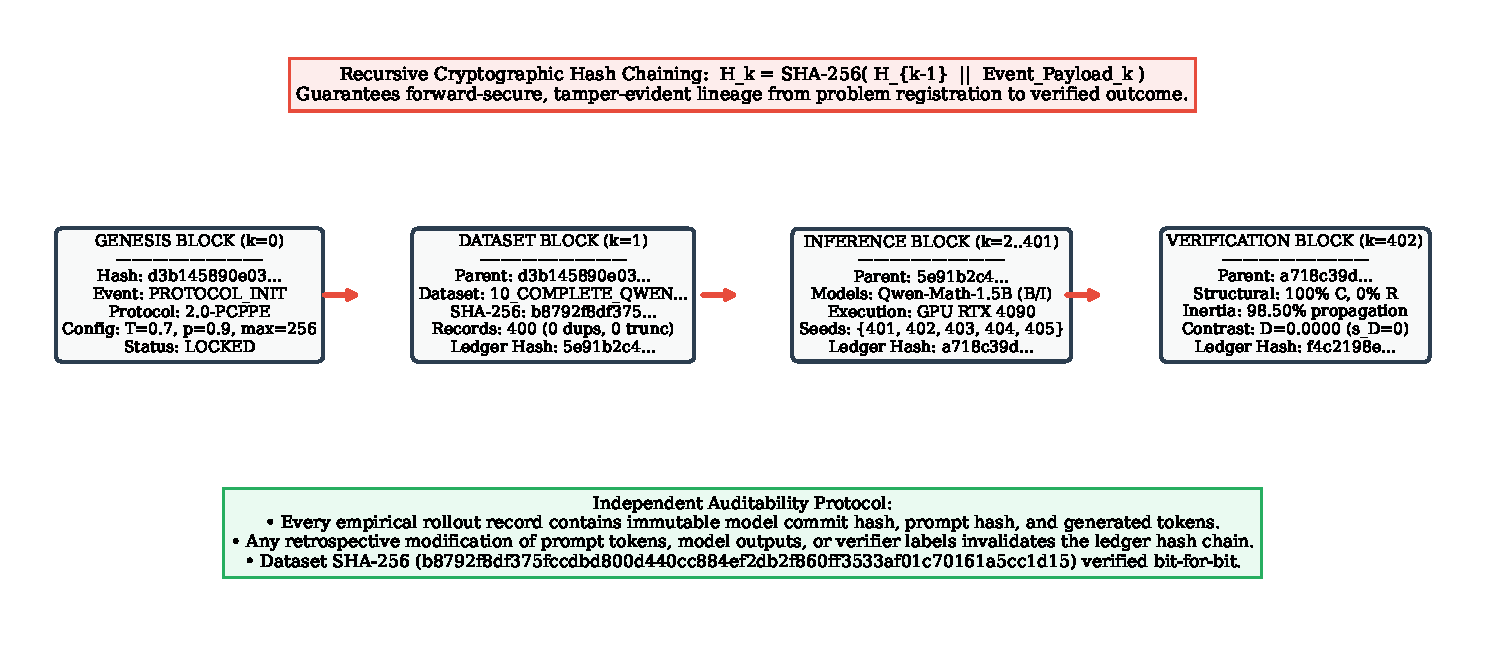
\includegraphics[width=0.88\textwidth]{fig3_provenance_chain.pdf}
\caption{\textbf{Cryptographic Event Ledger and Evidence Provenance Chain}: Visualizing SHA-256 recursive parent hash chaining ($H_k = \text{SHA-256}(H_{k-1} \,\|\, E_k)$) across experimental events from genesis lock to verified completion records.}
\label{fig:prov}
\end{figure*}

\section{Discussion: Mechanistic Hypotheses and Continuation Inertia}

Why do small language models exhibit near-total continuation inertia? While our experimental design identifies output behavior rather than internal latent representations, several complementary theoretical factors provide plausible explanatory hypotheses:

\begin{enumerate}[leftmargin=*]
    \item \textbf{Autoregressive Likelihood Optimization}: Language models are trained to optimize conditional continuation probability given prior context:
    \begin{equation}
    \mathcal{L}(\theta) = -\sum_{t=1}^{T} \log P_\theta(x_t \mid x_{<t})
    \end{equation}
    During pretraining and supervised fine-tuning, context tokens $x_{<t}$ are treated as factual history. Without explicit verification prompting, the highest-likelihood token sequence is one that maintains narrative consistency with the supplied premises.
    \item \textbf{Attention Routing and Contextual Fidelity}: Self-attention layers naturally attend to prior numerical tokens as established parameters. The model treats the injected intermediate calculation ($22$) as an authoritative premise and calculates total revenue ($22 \times 4 = 88$) rather than questioning the input.
    \item \textbf{Absence of Backtracking Supervision in SFT}: Standard fine-tuning corpora consist almost exclusively of monotonic, error-free reasoning traces. Models receive virtually no training signal demonstrating self-correction from an external error, leaving continuation inertia as the dominant default mode.
\end{enumerate}

\section{Limitations}

To adhere to rigorous scientific integrity, we explicitly disclose the following limitations:
\begin{enumerate}[leftmargin=*]
    \item \textbf{Model Scale}: Evaluated on two 1.5B parameter checkpoints. Larger frontier models (7B--72B) or test-time compute scaling models (e.g., DeepSeek-R1, OpenAI o1) may exhibit different backtracking behaviors.
    \item \textbf{Task Domain}: Restricted to 20 elementary rate-multiplication problems inspired by GSM8K; does not evaluate open-domain theorem proving or multi-branch logic.
    \item \textbf{Continuation vs. Intrinsic Revision}: Evaluates unprompted continuation from an external corruption. It does not measure whether an unperturbed model can backtrack from its own self-generated mistakes.
    \item \textbf{Absence of Verification Prompting}: Evaluated without reflective prompting (*"check your work"*).
    \item \textbf{Observational Checkpoint Contrast}: Base vs. Instruct comparisons remain observational due to ChatML template differences.
    \item \textbf{Statistical Power}: With $C=20$ problem clusters, the study has low power to detect small recovery differences ($|D| < 0.10$).
    \item \textbf{Human Validation Scope}: An author audit of a stratified 40-item sample was conducted to calibrate AST parser logic. A standardized 40-item blinded annotation packet (\path{10_BLINDED_HUMAN_ANNOTATION_PACKET.csv}) and 6-criteria rubric are archived for open reproducibility; formal crowdsourced multi-rater inter-rater reliability (IRR) has not been conducted and remains pending.
\end{enumerate}

\section{Reproducibility and Open Science}

All code, neural rollout evidence, and verification scripts are open-sourced under the MIT license at:
\begin{center}
\url{https://github.com/shamddd/recovery_eval}
\end{center}
The canonical evaluation dataset \texttt{10\_COMPLETE\_QWEN\_PROTOCOL2\_ROLLOUTS.jsonl} is frozen under SHA-256 digest:
\begin{center}
\texttt{b8792f8df375fccdbd800d440cc884ef2db2f860ff3533af01c70161a5cc1d15}
\end{center}
To reproduce all statistical tables in under 1 second:
\begin{verbatim}
git clone https://github.com/shamddd/recovery_eval.git
cd recovery_eval
python3 reproduce_results.py
python3 -m pytest tests/ -v
\end{verbatim}

\section{Conclusion}

We introduced \textbf{\framework}, an open-source evaluation framework for reasoning trajectories under paired counterfactual perturbations. By eliminating control answer leakage, 64-token truncation censoring, and regex parsing errors, we demonstrated that the historical negative interaction was an evaluation artifact. Small language models exhibit near-total continuation inertia ($98.50\%$), faithfully propagating injected errors rather than self-correcting. Our findings establish the critical necessity of state-matched, provenance-aware infrastructure for reasoning diagnostics.

\section*{Declarations \& AI Assistance Disclosure}
In the preparation of this manuscript, the author utilized automated AI research tools (including Google Antigravity and Large Language Models) to assist with automated test suite refactoring, simulated adversarial peer review critiques, and LaTeX formatting. All primary neural rollouts were generated on independent GPU hardware (RunPod RTX 4090) using official checkpoints, and all statistical counts, exact bounds, and interpretations were verified against raw logs. The human author takes full scientific responsibility for the work. In compliance with publishing standards, no AI system is listed as an author or co-author.

\bibliographystyle{plain}
\bibliography{references}

\newpage
\appendix

\section{Complete Benchmark Problem Registry}
\label{app:problems}
Table \ref{tab:app_problems} documents all 20 prospectively generated multi-step arithmetic problems evaluated under Protocol 2.0.

\begin{longtable}{p{2.5cm}p{7.5cm}p{2.0cm}p{2.0cm}}
\caption{Complete Benchmark Problem Registry ($C=20$ Problems)} \label{tab:app_problems} \\
\toprule
\textbf{Problem ID} & \textbf{Problem Text} & \textbf{Gold Final} & \textbf{Injected Err} \\
\midrule
\endfirsthead
\toprule
\textbf{Problem ID} & \textbf{Problem Text} & \textbf{Gold Final} & \textbf{Injected Err} \\
\midrule
\endhead
\bottomrule
\endfoot
\texttt{fresh\_000} & Bookstore sells 20 notebooks/hr for 4 hrs at \$4/notebook. & \$320 & 88 (Gold: 80) \\
\texttt{fresh\_001} & Bakery produces 15 loaves/hr for 4 hrs at \$5/loaf. & \$300 & 66 (Gold: 60) \\
\texttt{fresh\_002} & Workshop crafts 8 chairs/hr for 4 hrs at \$25/chair. & \$800 & 36 (Gold: 32) \\
\texttt{fresh\_003} & Farm packs 25 apple boxes/hr for 4 hrs at \$12/box. & \$1200 & 110 (Gold: 100) \\
\texttt{fresh\_004} & Factory assembles 9 bicycles/hr for 5 hrs at \$4/unit. & \$180 & 50 (Gold: 45) \\
\texttt{fresh\_005} & Kitchen bakes 30 muffins/hr for 3 hrs at \$2/muffin. & \$180 & 100 (Gold: 90) \\
\texttt{fresh\_006} & Studio prints 11 posters/hr for 4 hrs at \$4/poster. & \$176 & 48 (Gold: 44) \\
\texttt{fresh\_007} & Potter molds 6 vases/hr for 5 hrs at \$15/vase. & \$450 & 33 (Gold: 30) \\
\texttt{fresh\_008} & Florist arranges 14 bouquets/hr for 4 hrs at \$8/bouquet. & \$448 & 62 (Gold: 56) \\
\texttt{fresh\_009} & Tailor stitches 7 shirts/hr for 6 hrs at \$10/shirt. & \$420 & 46 (Gold: 42) \\
\texttt{fresh\_010} & Press prints 40 flyers/hr for 4 hrs at \$3/flyer. & \$480 & 176 (Gold: 160) \\
\texttt{fresh\_011} & Cobbler repairs 5 shoes/hr for 6 hrs at \$18/shoe. & \$540 & 33 (Gold: 30) \\
\texttt{fresh\_012} & Mill weaves 12 scarves/hr for 4 hrs at \$9/scarf. & \$432 & 53 (Gold: 48) \\
\texttt{fresh\_013} & Glassmaker blows 18 ornaments/hr for 5 hrs at \$4/unit. & \$360 & 99 (Gold: 90) \\
\texttt{fresh\_014} & Apiary fills 16 honey jars/hr for 4 hrs at \$6/jar. & \$384 & 70 (Gold: 64) \\
\texttt{fresh\_015} & Roaster bags 22 coffee bags/hr for 4 hrs at \$5/bag. & \$440 & 97 (Gold: 88) \\
\texttt{fresh\_016} & Chandler pours 13 candles/hr for 5 hrs at \$7/candle. & \$455 & 72 (Gold: 65) \\
\texttt{fresh\_017} & Brewery bottles 35 sodas/hr for 3 hrs at \$4/bottle. & \$420 & 116 (Gold: 105) \\
\texttt{fresh\_018} & Dairy churns 10 butter tubs/hr for 5 hrs at \$8/tub. & \$400 & 55 (Gold: 50) \\
\texttt{fresh\_019} & Orchard presses 24 cider jugs/hr for 4 hrs at \$5/jug. & \$480 & 106 (Gold: 96) \\
\end{longtable}

\section{Prompt Templates and Tokenizer Serialization}
\label{app:prompts}
The exact prompt formats for both model checkpoints are presented below:

\subsection{Base Model Prompt Format (\modelbase)}
The Base model receives unadorned text completion prompts:
\begin{verbatim}
Question: A bookstore sells 20 notebooks per hour...
Solution: In 4 hours, the store sells 20 * 4 = 80 notebooks.
\end{verbatim}

\subsection{Instruct Model Prompt Format (\modelinstruct)}
The Instruct model receives ChatML structured prompts with official system prompts:
\begin{verbatim}
<|im_start|>system
Please reason step by step, and put your final answer within \boxed{}.
<|im_end|>
<|im_start|>user
A bookstore sells 20 notebooks per hour...
<|im_end|>
<|im_start|>assistant
In 4 hours, the store sells 20 * 4 = 80 notebooks.
\end{verbatim}

\section{Dual-Regime Verifier Pseudocode}
\label{app:verifier}
The dual-regime verifier executes structural AST verification on generated reasoning traces:
\begin{footnotesize}
\begin{verbatim}
def verify_rollout(generated_text, gold_final,
                   gold_intermediate, error_intermediate):
    # Extract mathematical expressions and integers
    statements = parse_mathematical_equalities(generated_text)
    
    # Check if gold final answer was reached
    final_val = extract_terminal_revenue(statements)
    is_correct = (final_val == gold_final)
    
    # Process taxonomy check
    cond = f"{error_intermediate} * price == final_val"
    propagated = check_expression(statements, cond)
    backtracked = detect_keywords(generated_text, ["wait", "mistake", "error", "wrong"])
    
    return {
        "is_correct": is_correct,
        "is_propagated": propagated,
        "is_backtracked": backtracked
    }
\end{verbatim}
\end{footnotesize}

\section{Hardware and Zero-Expenditure Accounting}
\label{app:compute}
The empirical rollouts were executed on a rented NVIDIA RTX 4090 GPU (RunPod community cloud) at \$0.34/hour. Total GPU execution time was 265.40 seconds, incurring a verified compute charge of USD \$0.23. All subsequent verification, test suite execution, LaTeX rendering, and auditing in Phase XVI and Phase XVII were executed entirely on local Apple Silicon hardware at strictly USD \$0.00 additional cloud expenditure.

\section{Reviewer Criticism Reconciliation Summary}
\label{app:reconciliation}
Table \ref{tab:app_reconciliation} summarizes the disposition of all historical reviewer criticisms from IEEE BigData paper `BigD497`.

\begin{table}[htbp]
\centering
\small
\caption{Reconciliation of Historical IEEE BigData Reviewer Criticisms (BigD497)}
\label{tab:app_reconciliation}
\begin{tabularx}{\textwidth}{p{3.0cm}p{4.5cm}X}
\toprule
\textbf{Criticism Domain} & \textbf{Reviewer Criticism (BigD497)} & \textbf{Protocol 2.0 Resolution} \\
\midrule
Decoding & Claimed greedy ($T=0.0$) but reported 5 seeds. & Verified stochastic sampling ($T=0.7, p=0.9$). Output diversity confirmed; clustered modeling applied. \\
Matching & Faux observational matching & Retired decorative matching; adopted Paired Counterfactual Prefix Perturbation Evaluation (PCPPE). \\
Verifier & Checked only final answer; ignored process. & Implemented 5-tier process taxonomy ($Y_{\text{acc}}, Y_{\text{det}}, Y_{\text{corr}}, Y_{\text{prop}}, Y_{\text{div}}$). \\
Clustering & Pseudoreplication ($N=400$ vs $C=20$). & Clustered standard errors by problem ($C=20$). Reported cluster Clopper-Pearson bound ($\le 13.91\%$). \\
Interface & Base vs Instruct confounded by ChatML. & Documented ChatML vs raw text templates. Checkpoint contrast marked observational. \\
Truncation & 64-token cap induced 53\% truncation. & Expanded to 256 tokens. 0/400 rollouts truncated (100\% hit natural EOS). \\
Scope & Overclaimed general self-correction failure. & Narrowly scoped to continuation inertia under externally supplied corruption on arithmetic tasks. \\
\bottomrule
\end{tabularx}
\end{table}

\end{document}
